\chapter{The Communities}
\label{ch:02}



\begin{center}
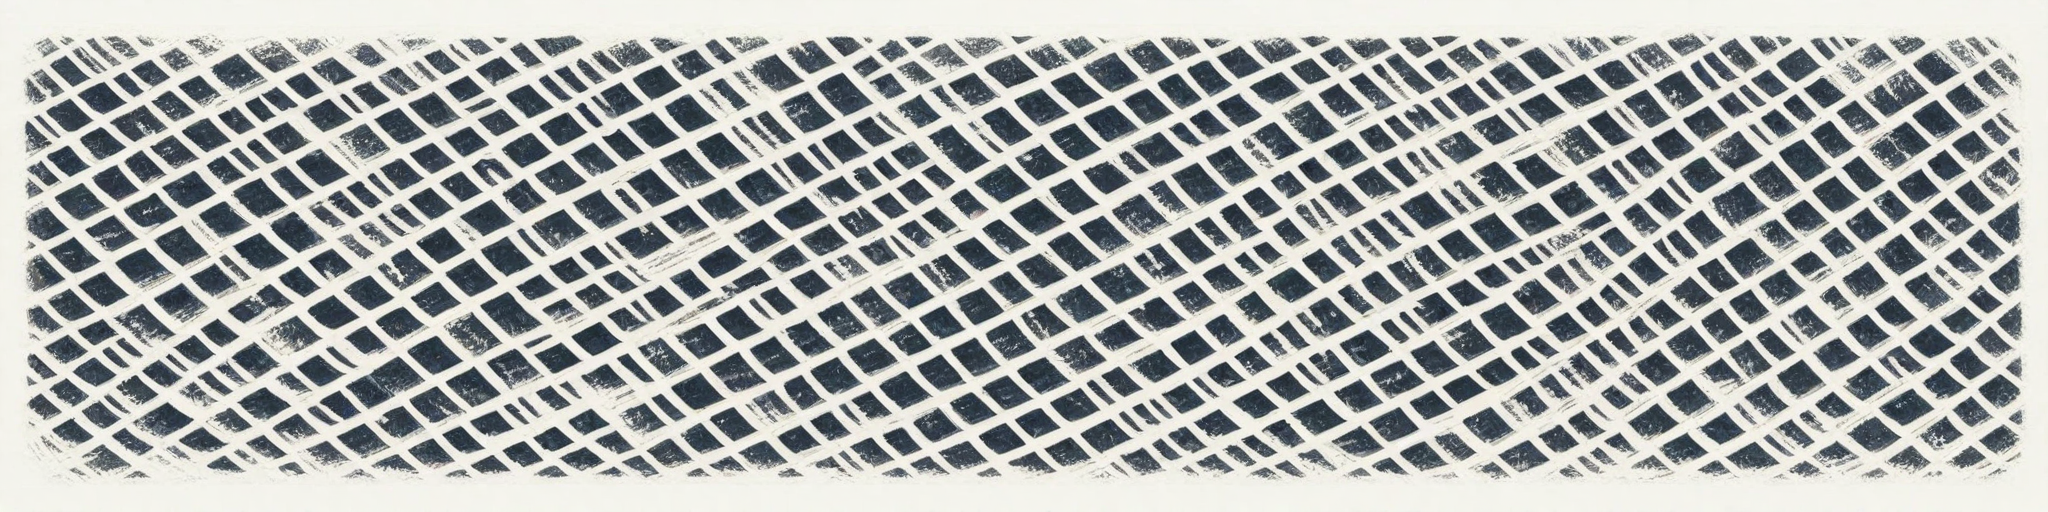
\includegraphics[width=\textwidth]{images/chapterImages/genesis_sketch_00054_.png}
\end{center}

Across the wide river, where the forest gave way to broken ground and exposed stone, another one worked.

He was larger than the Watcher, heavier in build, with darker feathers that showed bronze in direct sunlight. He stood in the middle of a vast flat area of weathered rock, surrounded by stones of various sizes. Some he had carried here over days. Others had always been here, part of the landscape, but he had moved them. Arranged them. Destroyed the arrangement. Begun again.

The current pattern spread across twenty body lengths of stone. Smaller rocks formed lines that curved and intersected. Larger ones marked specific points where the lines met or diverged. From the ground, it looked chaotic. Random, perhaps. The work of boredom or some inexplicable compulsion.

From above, had there been anything capable of flight large enough to achieve such height and perspective, the pattern would have revealed itself. Spirals that nested within spirals. Sequences of spacing that repeated with mathematical precision. Prime numbers encoded in the distances between stones. Fibonacci ratios in the curves.

The Builder—though no one called him that, though he had no name—nudged a stone half a body length to the left with his snout. Stepped back. Circled the entire formation, examining it from multiple angles. The mathematics was correct. He could feel it, the rightness of the ratios, the way each element related to the others in exact proportion.

But it was incomplete.

He began dismantling it.

Not violently. Methodically. Each stone picked up with care and moved to the formation's edge. The lines disappeared. The spirals dissolved. Within an hour, the flat stone was bare again except for the pile of stones at its perimeter.

He stood in the center of the empty space. Completely still for a long time. Then he picked up a stone and placed it. A different starting point. A different configuration. The same underlying mathematics, but expressed through a different geometry.

He would work on this one for three days before destroying it and beginning again.

\scenebreak

In the marshlands to the south, where the trees grew straight out of shallow water and the air hummed with insects, two of them sat facing each other.

They had been sitting this way for eleven days.

They were of similar size, similar build, their feather patterns almost identical. Whether they were mates or siblings or unrelated entirely was unclear. Perhaps it didn't matter. They sat precisely three body lengths apart, close enough that the space between them felt intentional, separated enough that they never touched.

Their eyes were open. They breathed. Sometimes one would shift slightly—a minor adjustment of weight distribution, a repositioning of the tail for better balance. The other would mirror the movement seconds later, or sometimes simultaneously. But mostly they simply sat.

To an observer, it might have looked like a standoff. A territorial dispute frozen in time, waiting for one to make the first move. Or perhaps a courtship ritual, some long pre-mating behavior programmed into their biology.

They weren't fighting. They weren't courting.

They were communicating.

It happened in ways too subtle for most creatures to detect. Micro-adjustments of posture that conveyed information. Shifts in breathing patterns that matched or deliberately diverged. Pheromone exchanges so dilute they might as well have been mathematical abstractions. The dilation of pupils. The angle of neck feathers. The precise timing of blinks.

Behind their eyes, vast datasets transferred between them. Observations accumulated over years. Patterns recognized in weather, in stellar positions, in the behavior of other creatures. Mathematical relationships tested and confirmed or disproven. One would pose a problem through nothing more than a slight cant of the head. The other would process, calculate, respond with a nearly imperceptible shift of weight that meant yes, no, or here is an alternative.

They had been in this clearing for eleven days and would remain for eighteen more before they moved. When they separated, each would carry information the other had possessed. The sum of their knowledge would be greater than its parts.

But to anything watching, they simply sat. Still as stones themselves. Waiting for something or nothing.

\scenebreak

Far to the north, where the forest climbed into foothills that would one day be mountains but were now just the beginning of elevation, a cliff face rose fifty body lengths above the canopy. The stone was soft here—sedimentary layers that held the impression of ancient seas, though seas had long since receded.

The Carver worked on this stone.

She was old. Older than most of her kind lived to be. Scars crossed her hide where feathers no longer grew. One eye was clouded, though the other remained sharp. She moved with care, each step deliberate not from precision but from the ache of aged joints.

She clung to the cliff face with her killing claws extended, gripping small ledges and crevices. Her hands worked at the stone. Scratching. Scoring. Wearing away layers with patient repetition.

The patterns she carved were intricate. Flowing lines that branched and rejoined. Circles that intersected other circles in specific ways. Sequences of marks—short, short, long, short, short, short, long, long—that repeated with variation. From a distance they looked like abstract art. Beautiful but meaningless.

Up close, they were something else.

Genetic sequences, though no one would call them that for millions of years. Molecular structures. Chains of information that, if read correctly, if understood in the right context, would unlock specific instructions. Modifications. Triggers.

She had been working on this cliff face for six years. She would work until she died, which would be soon. Others would continue her work, whether they understood it fully or simply felt the correctness of the patterns she had begun.

She paused in her carving, gripping the stone with three feet while one hand hung free. Her head tilted up, the good eye tracking something in the sky. A point of light that shouldn't be there. That was wrong in a way that made the calculations shift, made the patterns on the stone more urgent.

She returned to carving with increased intensity, though her movements remained precise. There was no time to waste on inefficiency.

\scenebreak

And elsewhere, scattered across the continent:

A young one stood in a streambed, arranging pebbles in complex geometries that the water would wash away by morning. She rebuilt the same pattern every evening anyway.

One of the massive long-necks stood at a forest edge, its small head moving back and forth with rhythmic precision, counting something invisible. It had been counting for three days. The number was important, though what it counted remained unclear.

A pack of hunters moved through tall grass, their formation maintaining exact geometric relationships even as they navigated obstacles. The spacing between them never varied by more than a body length. When one adjusted position, all the others compensated instantly.

In a cave network deep beneath the surface, one of them traced patterns in the soft mud walls. Spirals and branches and intersecting lines. The cave was too dark to see clearly, but the patterns never deviated. Perfect even in blindness.

\scenebreak

And near the Watcher's territory, though she had never directly encountered him, another one moved through the forest.

He was of her kind—same build, same size, similar feather patterns though his showed more brown tones where hers were gray. He moved with the same economical efficiency, the same precise placement of feet that disturbed nothing unnecessarily.

He had seen her, though she hadn't seen him. Had watched her from a ridge above her clearing as she stood for hours tracking the sky. Had observed her stone arrangement from a distance after she left. Had studied the geometry without touching it, understanding immediately what it represented even if he couldn't calculate to the same depth she clearly could.

He had his own work. His own patterns.

But he had begun ranging closer to her territory in the evenings. Not intrusive. Not threatening the space she clearly used. Just... closer.

He carried food sometimes—small mammals he had caught, more than he needed for himself. He cached the excess near the hollow tree where she roosted, far enough away that it wouldn't seem deliberate, close enough that she would find it.

She had found it. Had eaten it. Had shown no sign of acknowledgment.

He continued anyway.

Now he stood on a ridge overlooking the river valley, watching the sun descend. He would move to his own roosting site soon. But first he looked at the sky, finding the star point that was wrong, that didn't belong. His head tilted at precisely the same angle hers had that morning, though he couldn't have seen her do it. The angle was simply correct for optimal observation of that specific point.

He held the position for twenty minutes. Calculating what he could calculate. Knowing it wasn't enough, that his mind couldn't hold the full complexity the way some others clearly could. But contributing what he could to the collective understanding that existed without words, without formal structure, just distributed awareness shared through observation and imitation and subtle cues.

When he moved on, heading toward his roost, he adjusted his path slightly. Tomorrow he would range even closer to her territory. Tomorrow he would cache more food near her hollow.

Not courtship, exactly. Not yet.

Just proximity. Just offering what he could.

\scenebreak

Night fell across the continent. In hundreds of locations, in thousands of individual territories, they stopped their work and settled into roosts and dens and protected spaces. They slept the way their kind had always slept, with part of the brain always aware, always ready.

But in their dreams—if dreams were what those firing neural patterns could be called—the calculations continued. The patterns refined themselves. The observations integrated into larger frameworks of understanding.

The star point moved across the sky, following laws older than any consciousness that observed them. Gravity and velocity and the patient mathematics of orbital mechanics.

And below, distributed across an entire planet, an intelligence that had never spoken, never written, never built cities or tools, calculated its trajectory. Understood what it meant. Began, in their separate and collective way, to plan.

The stones remained where they had been placed. The patterns stayed carved and arranged and configured. Tomorrow they would continue. Tomorrow the work would grow more complex.

Tomorrow the star would be closer.

Not close enough to see the change with eyes alone. But close enough to feel it in the mathematics. Close enough to know.

Close enough to begin.

